\section{Einleitung}
\label{sec:einleitung}
	Um die "au"seren H"ullenelektronen zu untersuchen reicht es diese mit UV- und IR-Strahlung zu untersuchen. Zugang zu tieferliegenden Teilen der Atomh"ulle bekommt man jedoch nur mit der energiereichen R"ontgenstrahlung, deren Energiebereich sich von etwa $\SI{10}{\electronvolt}$ bis $\SI{100}{\electronvolt}$ erstreckt.
	\vspace{0.3cm}
	Zun"achst wird die Erzeugung der R"ontgenstrahlung und das resultierende Emissionsspektrum beschrieben. Anschlie"send wird deren Wechselwirkung mit Materie und den daraus resultierenden Absorptionsspektren betrachtet. Im letzten Teil ist das Verfahren zur Energie- und Intensit"atsmessung bei R"ontgenstrahlung interessant.

\section{Funktionsweise und theoretische Grundlagen}
\label{sec:funktionsweise}

	
	\subsection{Die Entstehung der R"ontgenstrahlung}
	\label{sub:entstehung}

		Wenn Elektronen in Materie eindringen, k"onnen sie in mehreren Ionisationsprozessen ihre kinetische Energie schrittweise, ohne Strahlung zu erzeugen, in W"arme umwandeln.
		Es kommt jedoch auch vor, dass ein Elektron in eine tiefere H"ulle eines Atoms eindringt und somit in den Wirkungsbereich des Kernfeldes kommt.
		Coulomb-Wechselwirkungen lenken das Elektron dabei von seiner geradlinigen Bahn abgelenkt.
		Beschleunigte Ladungen emittieren elektromagnetische Strahlung.
		Die E\-mis\-sions\-wah\-schein\-lich\-keit ist dabei proportional zur Kernladungszahl $z$.
		Das Energiespektrum der sogenannten Bremsstrahlung ist dabei kontinuierlich und reicht von null bis zu einem Maximalwert, der der gesamten kintischen Energie des gebremsten Elektrons entspricht.
		\\
		In Konkurrenz zum Abbremsprozess steht die Ionisation des Atoms in einer seiner inneren Schalen, welche jedoch instabil ist.
		Dabei muss das einfallende Elektron min\-des\-tens die Bindungsenergie des Elektrons besitzen, welches aus der Schale herausgeschlagen werden soll.
		Die R"uckkehr in den Grundzustand erfolgt dabei mit einer Relaxationszeit der Gr"o"senordung $\SI{e-8}{\second}$, wobei die L"ucken der Schalen von Elektronen h"oherer Schalen aufgef"ullt werden. 
		Das so entstandene "`Loch"' wird wiederum von einem Elektron einer noch h"oheren Schale aufgef"ullt.
		Dabei entsteht elektromagnetische Strahlung, deren Energiebetrag jedoch diskret ist und gegeben ist durch:

		\begin{equation}
			E_{\text{photon}} = h \nu = E_\mathrm{n} - E_\mathrm{m}. \label{gleich_1}
		\end{equation}
		\begin{center}
			$h$ = Planksches Wirkungsquantum, $\nu$ = Frequenz der Strahlung,\\
			$E_\mathrm{n}$ und $E_\mathrm{m}$ = Energieniveaus in der Elektronenh"ulle des Atoms.
		\end{center}
	
		{Da diese vom Matrial abh"angig ist, wird auch von charakteristischer R"ontgenstrahlung gesprochen.}
		
	\subsection{Die Erzeugung von R"ontgenstrahlung}
	\label{sub:erzeugung}

		Zur Erzeugung von R"ontgenstrahlung werden demnach schnelle Elektronen ben"otigt, welche "ublicherweise in einer R"ontgenr"ohre erzeugt werden, welche in Abb. \eqref{roentgenroehre} schematisch dargestellt ist.
		In einem evakuiertem Glaskolben erzeugt ein Gl"uhdraht durch thermische Emission freie Elektronen. 
		Diese werden von einer, sich gegen"uber der Kathode be\-find\-lich\-en, Kupferanode "uber ein elektrisches Feld angezogen und dadurch in Richtung der Anode beschleunigt.
		An dieser entsteht die R"ontgenstrahlung nach den in \eqref{sub:entstehung} beschriebenen Prozessen.

		\begin{figure}[htbp]
			\centering
			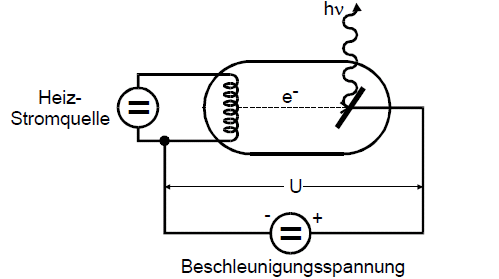
\includegraphics[width = 12cm]{img/Roentgenroehre.png}
			\caption{Schematischer Aufbau einer R"ontgenr"ohre \cite{anleitung}}
			\label{roentgenroehre}
		\end{figure}

	\subsection{Das Emissionsspekrum ohne Feinstruktur}
	\label{sub:ohnefein}

		Die intensit"at beschreibt die Zahl der pro Zeit- und Fl"acheneinheit einfallenden Quanten.
		Bei der Bremsstrahlung geht diese f"ur $E \rightarrow 0$ asymptotisch gegen null. Die maximale Energie $E_\mathrm{max}$ ergibt sich durch eine Energiebetrachtung und ist gleich der kinetischen Energie $E_\mathrm{kin}$.
		Daraus folgt:

		\begin{equation}
			E_\mathrm{max} = h\nu_\mathrm{max} = e_\mathrm{0}U. \label{gleich_2}
		\end{equation}
		\begin{center}
			$e_\mathrm{0}$ = Elementarladung.
		\end{center}

		Schwieriger sind die Linien des charakteristischen Spektrums zu berechnen, was mit Hilfe von Gleichung \eqref{gleich_1} m"oglich ist.
		Diese sind bekanntlich L"osungen der Schr"odinger-Gleichung. 
		Da es sich jedoch um ein System mit Viel-Elektron-Atomen handelt, l"asst sich das Problem auf eine sogenannte Einelektronanregung vereinfachen.
		Dabei wird angenommen, dass sich das "`emittierende"' Elektron in einem Coulomb Feld befindet, welches sich aus dem Kernfeld und den Feldern der restlichen H"ullenelektronen zusammensetzt.
		Dabei wird nicht die Kernladungszahl $z$ benutzt, sondern die Gr"o"se $z_\mathrm{eff}$ mit $z_\mathrm{eff} < z$, welche den Einfluss der Elektronen ber"ucksichtigt.
		Das emittierende Elektron besitzt damit die Potentielle Energie:

		\begin{equation}
			U = -\frac{z_\mathrm{eff} e_\mathrm{0}^2}{4 \pi \epsilon_\mathrm{0} r}. \label{gleich_3}
		\end{equation}
		\begin{center}
			$\epsilon_\mathrm{0}$ = Influenzkonstante, r = Orstkoordinate.
		\end{center}

		Es ergibt sich aus der Schr"odinger-Gleichung f"ur die Energie-Eigenwerte: 		
		\begin{equation}
			E_\mathrm{n} = - R_\infty z_\mathrm{eff}^2 \frac{1}{n^2}. \label{gleich_4}
		\end{equation}
		\begin{center}
			$R_\infty$ = Rydberg-Energie, n = Hauptquantenzahl.
		\end{center}

		Dabei handelt es sich um eine g"ultige N"aherung f"ur kleine $z$.
		Eine bessere N"aherung wird im n"achsten Abschnitt beschrieben.
		Somit ergibt sich beim "Ubergang von der m-ten auf die n-te Schale der Energiebetrag:

		\begin{equation}
			h \nu_\mathrm{m,n} = R_\infty z_{\mathrm{eff}_\mathrm{m,n}}^2 \left( \frac{1}{n^2} - \frac{1}{m^2} \right). \label{gleich_5}
		\end{equation}

		F"ur $n < m$ kann nun durch Einsetzen aller nat"urlicher Zahlen in Gleichung \eqref{gleich_5} die Lage des charakteristischen Spektrums errechnet werden.
		Die Linien k"onnen nun anhand ihrer Hauptquantenzahl benannt werden, wobei $n = 1$ aus historischen Gr"unden als K-Schale bezeichnet wird und alle weitern f"ur $1 < n$ dem Alphabet folgend L,M,N,O,usw. Schale genannt werden. 

		\begin{figure}[htbp]
			\centering
			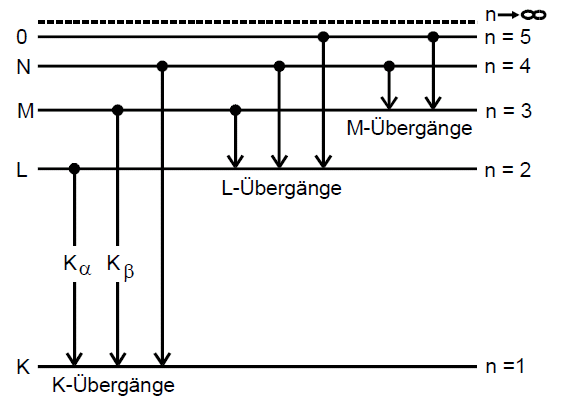
\includegraphics[width = 12cm]{img/Roentgenuebergaenge.png}
			\caption{M"ogliche R"ontgen"uberg"ange in einer Elektronenh"ulle ohne Feinstruktur. \cite{anleitung}}
			\label{roentgenuebergaenge}
		\end{figure}

		Abbildung \eqref{roentgenuebergaenge} zeigt die ersten Schalen und die m"oglichen "Uberg"ange auf diese. Die L"ange der Strahlung ist ein Ma"s f"ur die Energie der Strahlung.
		Im Vergleich zu optischen Spektren, welche durch Elektronenspr"unge in den "au"seren H"ullen verursacht werden, ergibt sich ein R"ontgenspektrum nur bei "Uberg"angen in den inneren H"ullen.
		Da diese meist nicht von der Bindung zu anderen Atomen betroffen sind, verschiebt sich das Spektrum monoton, wie in \eqref{gleich_5} beschrieben, zu h"oheren Frequenzen.
		Bei optischen Spektren hingegen ist eine Periodizit"at zu erkennen.

	\subsection{Emissionsspektrum mit Feinstruktur}
	\label{sub:emissionsspektrum_mit_feinstruktur}
	
		Durch das Betrachten der Feinstruktur gelingt eine bessere Betrachtung der Zu\-sam\-men\-h"an\-ge.
		Die Sommerfeldsche Feinstrukturformel, welche sich aus der St"orungsrechnung ergibt, bietet gerade bei gr"o"seren $z$ eine bessere N"aherung als \eqref{gleich_4}:

		\begin{equation}
			E_\mathrm{n,j} = -R_\infty \left(z_\mathrm{eff1}^2 \frac{1}{n^2} + \alpha^2 z_\mathrm{eff2}^4 \frac{1}{n^3} \left( \frac{1}{j + \frac{1}{2}} - \frac{3}{4n} \right) \right).\label{gleich_6}
		\end{equation}
		\begin{center}
			$\alpha$ = Sommerfeldsche Feinstrukturkonstante, und\\
			j = Gesamtdrehimpulszahl; \\
			Zusammensetzung aus der Bahndrehimpulszahl $l$ und der Spinquantenzahl $s = \frac{1}{2}$ mit\\
			$j = l + \frac{1}{2}$ oder $j = l - \frac{1}{2}$.
		\end{center}

		Es werden hier die effektiven Kernladungszahlen mit den Abschirmzahlen $\sigma$ und $s$ angegeben:

		\begin{eqnarray*}
			z_\mathrm{eff1} &=& z - \sigma,\\
			z_\mathrm{eff2} &=& z - s.
		\end{eqnarray*}

		Diese gr"o"sen beschreiben die Schw"achung des Kernfeldes durch die Elektronen, welche nicht an der Emission beteiligt sind.
		Die Abschirmzahl $\sigma$ wird dabei haupts"achlich durch die H"ul\-len\-e\-lek\-tro\-nen bestimmt, die ihr Ladungsverteilungsmaximum innerhalb der n-ten Schale haben.
		Dabei ist jedoch der Einfluss der "au"seren Elektronen nicht zu vernachl"assigen und es w"achst bei gleichem $n$ mit $z$.
		Es wird als "`Konstante der vollst"andigen Abschirmung"' bezeichnet.
		Die "`Konstante der "au"seren Abschirmung"' $s$ wird durch die Anzahl der Elektronen bestimmt, welche sich innerhalb der n-ten Schale befinden.
		Dabei ist kaum eine $z$-Ab\-h"an\-gig\-keit festzustellen.
		Die Abschirmzahlen $s$ und $\sigma$ h"angen stark von $n$ und $l$ ab.
		Damit ergibt sich f"ur \eqref{gleich_6}:

		\begin{equation}
			E_\mathrm{n,j} = -R_\infty \left( (z - \sigma_\mathrm{n,l})^2 \frac{1}{n^2} + \alpha^2 (z - s_\mathrm{n,l})^4 \frac{1}{n^3} \left( \frac{1}{j + \frac{1}{2}} - \frac{3}{4n} \right) \right). \label{gleich_7}
		\end{equation}

		F"ur die Hauptquantenzahl $n$ ergeben sich nur mehrere $l$ und $j$-Werte, wodurch es zu einer Feinstruktur-Aufspaltung kommt.
		Mit der "Uberlegung:

		\begin{eqnarray*}
			l_\mathrm{max} = n - 1
		\end{eqnarray*}

		ergibt sich f"ur die K-Elektronen kein Bahndrehimpuls, sondern nur ihr Eigendrehimpuls (Spin). 
		Daher folgt f"ur die K-Elektronen $j = \frac{1}{2}$ und damit dass sie keine Fein\-struk\-tur\-auf\-spal\-tung besitzen.
		F"ur die L-Schale mit $l = 0$ und $l = 1$ folgt f"ur die Kombinationen: [$j = \frac{3}{2}, l = 1$], [$j = \frac{1}{2}, l = 1$], [$j = \frac{1}{2}, l = 0$].
		Damit besitzt die L-Schale drei Unterniveaus.
		Mit analoger Rechnung kann man f"ur die M-Schale 5 Unterniveaus bestimmen.
		Anschaulich wird dies in Abbildung \eqref{roentgenfein} dargestellt.

		\begin{figure}[htbp]
			\centering
			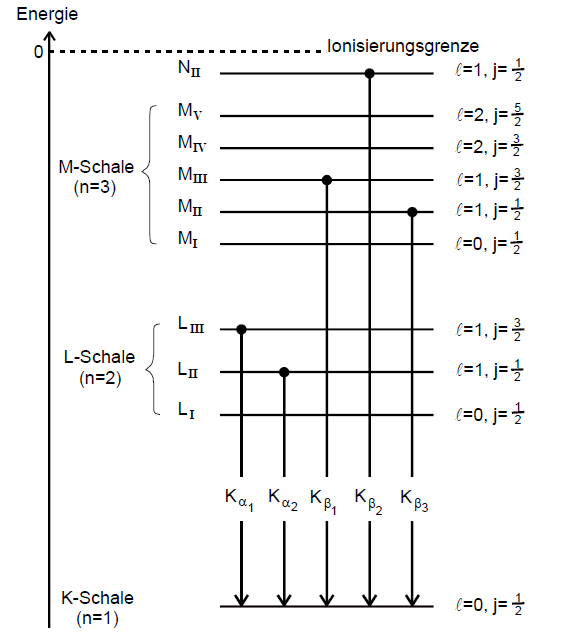
\includegraphics[width = 12cm]{img/Roentgenuebergaengefein.png}
			\caption{Feinsktruktur-Aufspaltung in einer Elektronenh"ulle. \cite{anleitung}}
			\label{roentgenfein}
		\end{figure}	

		Es gibt f"ur die Existenz an Kombinationen zwei grundlegende Einschr"ankungen: 
		1. $\Delta l$ \le $|1|$ sein darf und 2. die "Ubergangswahrscheinlichkeit f"ur $\Delta n$ \ge 3 nimmt drastisch ab. 
		Damit ergibt sich aus \eqref{gleich_8} f"ur den "Ubergang zwischen zwei Niveaus mit den Quantenzahlen $n$,$l$,$j$ und $n'$, $l'$, $j'$:	

		\begin{align}
		\begin{split}
			E = & -R_\infty \left( \frac{(z - \sigma_\mathrm{nl})^2}{n^2} - \frac{(z - \sigma_\mathrm{n'l'})^2}{n'^2} +  \alpha^2 \frac{(z - s_\mathrm{nl})^4}{n^3} \left( \frac{1}{j + \frac{1}{2}} - \frac{3}{4n} \right) - \right. \\& \left. - \alpha^2 \frac{(z - s_\mathrm{n'l'})^4}{n'^3} \left( \frac{1}{j' + \frac{1}{2}} - \frac{3}{4n'} \right) \right) . \label{gleich_8}
		\end{split}
		\end{align}

		Das Ziel dieses Experiments ist es f"ur verschiedene Atome die Abschirmzahlen $\sigma$ und $s$ zu bestimmen.
		Der Weg "uber die Energien des Emissionsspektrums ist allerdings daf"ur nur bedingt geeignet.
		Ein besserer Weg wird im n"achsten Kapitel betrachtet.

	\subsection{Das Absorptionsspektrum}
	\label{sub:das_absorptionsspektrum}
	
		Beim Durchgang durch Materie tritt eine Schw"achung der Strahlungsintensit"at auf.
		Diese ist haupts"achlich material- und energieabh"angig und tritt meist durch Absorption aber auch in geringerem Ma"se durch Streuung der R"ontgenstrahlung auf. 
		Die Absorption entfernt ein H"ullenelektron eines Atoms aus seiner Bindung und wird auch als "`innerer Photoeffekt"' bezeichnet:

		\begin{equation}
			h\nu = E_\mathrm{B} + E_\mathrm{kin}. \label{gleich_9}
		\end{equation}

		Aus \eqref{gleich_9} ergibt sich, dass die Energie des R"ontgenquants ($h\nu$) mindestens gleich der Bin\-dungs\-en\-er\-gie des H"ullenatoms ($E_\mathrm{B}$) sein muss, damit der Prozess m"oglich ist.
		"Ubersch"ussige Energie wird in Form von kinetischer Energie an das Elektron weitergegeben.
		Die Wahr\-schein\-lich\-keit f"ur die Absorpion ist proportional zur Kernladungszahl $z$ des Absorbermaterials und der Quantenenergie $h\nu$.
		Im Energiebereich unter $\SI{100}{\kilo\electronvolt}$ gilt die grobe N"aherung f"ur den Absorptionskoeffizienten $\mu$:
		
		\begin{equation}
			\mu \propto z^5 E^{-3.5}. \label{gleich_10}
		\end{equation}

		Wenn es einem Quant gelingt ein Elektron aus der H"ulle zu schlagen ergibt sich f"ur die energetische Betrachtung der K-Schale nach \eqref{gleich_6}:

		\begin{equation}
			h\nu_{\mathrm{K}_\mathrm{Abs}} = E_{1,\frac{1}{2}} - E_\infty = R_\infty \left( (z - \sigma_{0,1})^2 + \alpha^2 (z-s_{1,0})^4 \frac{1}{4} \right). \label{gleich_11}
		\end{equation}

		Innerhalb der K-Schale befinden sich jedoch nur wenig Elektronen, wodurch $s_{0,1}$ in \eqref{gleich_9} verschwindet und sich $\sigma_{0,1}$ aus einer Messung von $h\nu_{\mathrm{K}_\mathrm{Abs}}$ berechnen l"asst.
		An dem Beispiel der 3 L-Absorptionslinien soll eine Weitere M"oglichkeit zur Berechnung der Abschirmzahlen verdeutlicht werden.
		Nach \eqref{gleich_6} ergibt sich:

		\begin{eqnarray*}
			h \nu_\mathrm{L,abs,I} = E_{2,0,\frac{1}{2}} - E_\infty &=& R_\infty \left( \frac{(z-\sigma_{2,0})^2}{8} + \alpha^2 \frac{z - s_{2,0}}{8} \frac{5}{8} \right),\\
			h \nu_\mathrm{L,abs,II} = E_{2,1,\frac{1}{2}} - E_\infty &=& R_\infty \left( \frac{(z-\sigma_{2,1})^2}{4} + \alpha^2 \frac{z - s_{2,1}}{8} \frac{5}{8} \right),\\
			h \nu_\mathrm{L,abs,III} = E_{2,1,\frac{3}{2}} - E_\infty &=& R_\infty \left( \frac{(z-\sigma_{2,1})^2}{4} + \alpha^2 \frac{z - s_{2,1}}{8} \frac{1}{8} \right),\\
			\Rightarrow \qquad h\nu_\mathrm{L,abs,II} - h\nu_\mathrm{L,abs,II} &=& R_\infty \alpha^2 \frac{(z - s_{2,1})^4}{16}.
		\end{eqnarray*}

		Daraus l"asst sich nun die Abschirmzahl $s_{2,1}$ berechnen.
		Experimentell bestrahlt man das zu untersuchende Material mit monoenergetischen R"ontgen-Quanten und misst die Intensit"at der durchgehenden Strahlung in Abh"angigkeit von der Energie.
		Hiernach erh"alt man eine Kurve, wie sie in Abbildung \eqref{Absorption} idealisiert dargestellt ist.

		\begin{figure}[htbp]
			\centering
			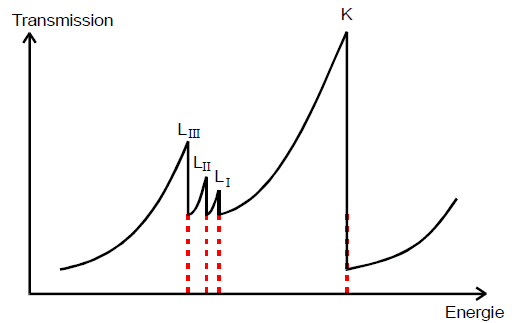
\includegraphics[width = 12cm]{img/absorption.png}
			\caption{Ein typisches R"ontgen-Absorptionsspektrum mit K- und L- Kanten. \cite{anleitung}}
			\label{Absorption}
		\end{figure}

		Nach \eqref{gleich_10} nimmt der Absorptionskoeffizient $\mu$ monoton mit der Quantenenergie ab und damit die Transmission zu.
		Sobald die Quantenenergie ausreicht, um ein Elektron he\-raus\-zu\-schla\-gen entsteht im Idealfall eine Unstetigkeit der Kurve, was als Absorptionskante bezeichnet wird.
		Diese ist identisch mit der Ab\-sorp\-tions\-e\-nergie $h\nu_\mathrm{abs}$.
		F"ur die K-Schale existiert aufgrund fehlender Feinstruktur nur eine K-Kante.
		Die L-Schale hingegen liefert 3 Ab\-sorp\-tions\-kan\-ten deren Energien berechnet werden k"onnen und so $s_{2,1}$ berechnet werden kann.\\
		Auf die Streuung der R"ontgenstrahlung in Form des Compton-Effekts und die Entstehung von neuen Quanten durch Fluoresenz-Strahlung wird hier nicht weiter eingegangen. Es ist jedoch zu erw"ahnen, dass diese nur bei Atomen mit $z < 13$eine Rolle Spielt.
		Im Experiment haben wir jedoch keine so leichten Atome.

	\subsection{Messung von Intensit"at und Energie der R"ontgenstrahlung} 
	\label{sub:messung_von_intensit_at_}
	
	Die Intensit"at der R"ontgenstrahlung ist proportional zur Messgr"o"se der Quanten pro Fl"achen- und Zeit-Einheit.
	Aus diesem Grund wird das einfach zu handhabende Geiger-M"uller-Z"ahlrohr zur Messung der Intensit"at verwendet. Dabei wird die ionisierende Wirkung der R"ontgenstrahlung ausgenutzt.
	Die Energie kann aus den Welleneigenschaften der R"ontgenstrahlung berechnet werden.
	Wenn R"ontgenstrahlung in Kristalle eindringt treten In\-ter\-fe\-renz\-er\-schei\-nung\-en auf.
	Dies ist der Fall, da Kristalle eine r"aumlich periodische Anordnung von Atomen besitzen und die Strahlung an ihnen elastisch gestreut wird. Dies wird in Abbildung \eqref{interferenz} verdeutlicht. 
	Konstruktive Interferenz tritt nur bei Gangunterschieden von ganzzahligen vielfachen von $\lambda$ auf.

	\begin{figure}[htbp]
		\centering
		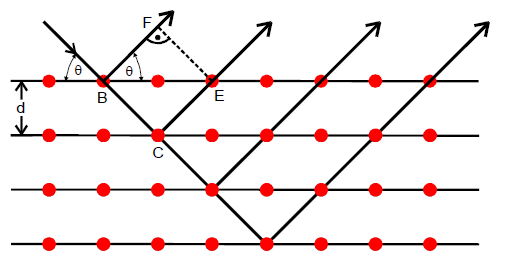
\includegraphics[width = 12cm]{img/interferenz.PNG}
		\caption{Zweidimensionales Kristallgitter zur Veranschaulichung der Interferenzbedingung. \cite{anleitung}}
		\label{interferenz}
	\end{figure}

	Die Winkel $\theta$, bei welchen stark erh"ohte Intensit"aten gemessen werden k"onnen, lassen sich mit Hilfe der Bragg'schen Reflexionsbedingung berechnen:

	\begin{equation}
		n \lambda = 2 d \sin(\theta); n = 1,2,3,\ldots (\text{Interferenzordnung}). \label{gleich_12}
	\end{equation}

	Mit der Beziehung

	\begin{equation}
		E = h \nu = h \frac{c}{\lambda}
	\end{equation}

	l"asst sich die R"ontgen-Quantenenergie in \eqref{gleich_12} einsetzen:

	\begin{equation}
		E = \frac{hc}{\lambda} = \frac{hcn}{2d\sin(\theta)}. \label{gleich_13}
	\end{equation}

	Man hat nun einen Zusammenhang zwischen der R"ontgen-Energie $E$ und dem Beugungswinkel $\theta$ bei gegebenem Netzabstand $d$ und Interferenzordnung $n$.
	Es ist nun also m"oglich "uber die Messung der Beugungswinkel direkt die Energie der R"ontgen-Quanten zu ermittelt. 
	Au"serdem kann mit Hilfe der Bragg-Reflexion an einem Kristall aus einer polyenergetischen Strahlung eine nahezu monoenergetische Strahlung erzeugt werden.